\section{Introduction}

The end of the 20th century gave rise to a need to quickly obtain information on the web. As a result of this, search engines were developed and are one of the most common methods to find information online today. Competition between different search engines has been present since the start, but Google has long ruled the market. Its has become widely used because its algorithms have outperformed those of other search engines. Not all of the algorithms that Google is using are publicly available, but those that are known have been present through decades, such as TF-IDF, BM25, PageRank and query likelihood ranking.

The aim of this report is to explore existing algorithms for information retrieval (IR) and how they perform against each other. To evaluate these algorithms in a tractable sized test environment, we implemented a search engine on the "cs.ucl.ac.uk" domain. The application includes implementations of several ranking algorithms, a variety of preprocessing techniques and data transformations as well as an evaluation of the results. The search engine application built for this project was implemented in Python and can be found on \url{github.com/navohu/IRDM_GROUP27}.\footnote{All instructions for running the application can be found in the README file of the repository.} Initially, our expectations for the project were to produce results that showed the difference of the current working algorithms, as well as an implementation of a deep learning algorithm. However, since our project only included a search on the CS domain and our test set is limited in size, the amount of data might not be sufficient for a deep learning approach.

This report will first discuss influential related work within the field of information retrieval. It will then move on to describe the methodology involved in creating the search engine: steps such as setting up an inverted index, programming the crawler and implementing the algorithms. After the methodology section we will introduce the methods and metrics we used in evaluating our algorithms. Finally, we will analyse our results and provide a discussion about the project, its limitations and potential expansions.


\section{Related Work}
Retrieving and ranking results in a search engine can be done through many different algorithms. In this section, we will explore the literature covering two categories of ranking algorithms: probabilistic and non-probabilistic. We will then investigate how the performance of an algorithm is commonly evaluated given a test set. Furthermore, we will review Deep Learning, a new topic that has caught attention within information retrieval, and how it can be used in search engines.

Today, web search is a tool that individuals, universities and businesses use on a daily basis. Many of these retrieval systems fall under traditional information retrieval. The first web search engine was created in 1993, but soon the renowned search engine Google was created by Larry Page and Sergey Brin. The feature that made Google better than its competitors was an algorithm called PageRank introduced by Page in 1998 \cite{brin1998anatomy}. He describes PageRank as "an objective measure of [a website's] citation importance that corresponds well with people's subjective idea of importance." This ranking algorithm is still used by Google today.

Another method of ranking the importance of a website was developed by Kleinberg in 1999 \cite{kleinberg1999authoritative}. He proposed a link analysis algorithm called HITS. It involves identifying hubs and authorities in a web graph, where hubs serve as large directories without specific authoritative information, while authorities hold important information. % TODO: clarify?

Both PageRank and HITS are algorithms that rank the importance of a page, but do not take a query into consideration. Hence, these algorithms are good for supplementing rankings returned by algorithms that take the query into consideration. Within query-dependent rankers, one of the earliest and simplest non-probabilistic algorithms was the Standard Boolean model introduced by Fayen \cite{lancaster1973information}. Since this algorithm is based on an exact match between the query terms and the document content, it will often either return too many or too few documents. This simple model was improved upon with more sophisticated algorithms such as the Vector Space Model \cite{salton1975vector}, Term Frequency -- Inverse Document Frequency (TF-IDF) \cite{salton1983mcgill}, and query likelihood language models \cite{zhai2001model} among others. They all have a goal of retrieving the most relevant documents for a given query. \\

IR research has always had a strong emphasis on measuring the efficacy of an IR system. This includes estimating the relevance of documents retrieved by a search engine relative to the user's information need. Evaluation is important in order to assess the performance of the system, measure the differences of multiple systems, and to learn the faults of a system such that IR methods can be improved in the future. The Text Retrieval Conference (TREC) supports and influences the IR community by providing evaluation infrastructure. The famous infrastructure for evaluation, trec\_eval, is used for all ad hoc tasks in TREC \cite{voorhees:evaluation}. Two of its measurements are precision and recall, first developed by Sparck-Jones \cite{jones1981information}. This type of evaluation is based on a document collection that includes documents classified as relevant or non-relevant, based on a set of queries.

On the other hand, work on IR evaluation has shown that defining relevance is very hard when it comes to "real" users \cite{mizzaro1997relevance}. Therefore, another method of capturing user interactions with a search engine is Transaction Log Analysis (TLA). It is based on creating transaction logs to recognise attributes within the search process. It's a way of measuring the searcher's actions, the interaction between the user and the system along with the results \cite{glaser1967discovery}. 

Having a stable and robust test collection is an important part of evaluation. This has resulted in a connected community where researchers have shared test collections with each other. Mark Sanderson emphasises the power of good test collections used in conjunction with evaluation measures \cite{sanderson:evaluation}. Evaluation methods used by Sanderson include Discounted Cumulative Gain (DCG) and normalised DCG (nDCG). DCG is often used to measure the ranking quality and the effectiveness of web-based search engines specifically. The algorithm measures the \textit{gain} of a document based on its position in the list. nDCG normalises the gain across queries by sorting the relevant documents by their relative relevance. \\

The very popular subject Deep Learning has also been used in web search engines. Huang et al. propose a deep structured semantic model that is trained by trying to reach the maximum conditional likelihood of a clicked document given a query \cite{huang2013learning}. The idea is based on click-through data collected which is used to feed the model in order to learn which pages are relevant to a query. Another paper by Deng et al. used deep stacking networks (DNS) in order to perform a parallel and scalable relevance prediction on an IR task \cite{deng2013deep}. It outperforms previous well known machine learning ranking algorithms such as LambdaRank and LambdaMART \cite{burges2010ranknet} in normalised DCG. 

%Many of these algorithms are commonly used in web search today and the rest of the report will explore how some of these techniques can be used in a search engine. A comparison between different methods will also be provided.


% section related_work (end)


\section{Experiments} % (fold)
\label{sec:experiment}

This section will present our overall methodology in building a search engine. Our methodology is freely and easily adaptable since it uses open source Python libraries and free-tier instances of Amazon Web Services Elastic Compute Cloud (EC2) and Relational Database Service (RDS). There are five main algorithms that have been implemented and contrasted in this project: Boolean Retrieval, TF-IDF, BM25, query likelihood estimation and PageRank. The assortment of algorithms was chosen after a thorough examination of the current literature in the field. We wanted to both test algorithms that have been shown to be very accurate and include some that are less advanced in order to provide a full overview of the the most known algorithms in the field, and cover the main differences between them. 

\subsection{Dataset Description} % (fold)
\label{sub:dataset_description}

The search engine is dealing with two core datasets: the crawled web pages and the test set for evaluation. The crawled web pages are specifically modified and transformed for use. Examples of this include creating an inverted index based on the content of the crawled web pages or producing an adjacency matrix based on the relationship between pages. 

The test set was manually created in order for us to evaluate the performance of our search engine. Two main categories were produced: one with navigational queries and another with informational queries. This means that the first set is specifically made up of queries where the user is looking for \emph{one} specific document (navigational), while the other set is created with the intention of measuring the capability of the search to retrieve as many relevant documents as possible (informational). Both test sets included queries as well as relevant documents related to the queries so that recall can be calculated. The composition of each test dataset is shown in Table \ref{dataset-table}, and the test sets in their entirety can be found in the \emph{queries} subfolder of our GitHub repository.  A justification for the choice of queries follows in section \ref{ssub:evaluation_queries}.

\begin{table}[H]
\centering
\caption{Composition of test datasets}
\label{dataset-table}
\resizebox{\columnwidth}{!}{%
\renewcommand{\arraystretch}{1.2}
\begin{tabular}{|c|c|c|c|}
\hline
Query & Total labels & Relevant & Non-relevant \\ \hline
\textbf{Informational} \\ \hline
degree & 152 & 87 & 65 \\ \hline 
Jun Wang & 101 & 30 & 71 \\ \hline
alphaGO & 30 & 4 & 26 \\ \hline
\textbf{Navigational} \\ \hline
moodle & 69 & 2 & 67 \\ \hline
information retrieval and data mining & 96 & 62 & 34 \\ \hline
computer graphics syllabus & 119 & 75 & 44\\ \hline
bioinformatics home page & 69 & 36 & 33 \\ \hline
\end{tabular}%
}
\end{table}

% subsection dataset_description (end)

\subsection{Indexing} % (fold)
\label{sub:methods}
A well-designed index is central to search engine performance. Before we could experiment with ranking algorithms, we had to set up cloud computing infrastructure for our index database, define the search domain to crawl, design a database schema and populate it with indexed data. The design decisions we made in the process are highlighted below. %The methodology includes a wide range of steps and exploration in order to build our search engine. These will be presented here.

\subsubsection{AWS Database \& Server Setup} % (fold)
\label{ssub:database_and_server_setup}

The search engine is run on an Amazon EC2 instance that provided secure and resizeable computing capacity. It is usually good practice to run heavy loaded applications -- such as a search engine -- on a cloud computing service. As a rule, there are more computing resources available, and these are more scalable and robust than on a local machine. Another advantage is that it's possible to set up a database instance which can be accessed by anyone. Our project is using a PostgreSQL database within RDS which can be accessed by the search engine running on either the EC2 server or a local machine outside AWS, if needed. However, due to geographical proximity of AWS services, faster performance can be observed from the EC2.\\

%We designed our database schema in such a way that it would be easy for our application to access the data when processing the rankings. To reduce redundancy and the risk of inconsistency, website links, content words and titles are each only stored once and referenced by foreign key IDs in other tables.
We designed our database schema with expandability, consistency, and ease of access in mind. It is mainly made up of tables \emph{cs\_sites}, \emph{cs\_dictionary} and \emph{cs\_word\_occurrence}, prefaced by \emph{cs} to allow further domains to be readily added. Furthermore, the database contains \emph{raw} dictionary and word occurrence tables (with the word \emph{raw} referring to unprocessed document terms), which can be used to isolate the effect of stopping and stemming on the final results.

Our crawler writes to \emph{cs\_cites}, built to hold the titles, URLs and unique IDs of web pages within the CS domain.
Based on these URLs, an inverted index is created, consisting of a dictionary that maps words to their IDs and collection-wide frequencies, and of a word occurrence table, which lists $word\_id$ -- $document\_id$ pairs and their frequencies. After the index is constructed, \emph{cs\_sites} is supplemented with document length and pagerank data.

% subsubsection database_and_server_setup (end)

\subsubsection{Crawling} % (fold)
\label{ssub:crawling}

The crawling was done through an open source platform called Scrapy written in Python.\footnote{https://scrapy.org} This platform is given a start URL "\url{www.cs.ucl.ac.uk}", on the outgoing links of which it performs a depth-first-search on all links containing the "\url{cs.ucl.ac.uk}" domain. This would include pages such as "\url{www.cs.ucl.ac.uk/home}", and "\url{www.wiki.cs.ucl.ac.uk}". We set a \emph{maximum depth} of the crawler because we found some links that were extremely long only contained details of the internal index of the CS website that were practically never opened by visitors to the website. The crawler also made sure not to crawl already crawled links. In the graph in Figure \ref{fig:graph} we can see an example where some links are pointing back to the root. These links would therefore not be crawled again.

\begin{figure}[!h]
\centering
\begin{tikzpicture}[-latex ,auto ,node distance =3cm and 2cm ,on grid ,
                    semithick , state/.style ={ circle ,top color =white , 
                    bottom color = white!20 , draw, black , 
                    text=black , minimum width =1 cm}]
\node[state] (C) {$cs.ucl.ac.uk/home$};
\node[state] (A) [above left=of C] {$cs.ucl.ac.uk$};
\node[state] (B) [above right =of C] {$cs.ucl.ac.uk/research$};
\path (A) edge [loop left] node[left] {} (A);
\path (C) edge [bend left =25] node[below =0.15 cm] {} (A);
\path (A) edge [bend right = -15] node[below =0.15 cm] {} (C);
\path (A) edge [bend left =25] node[above] {} (B);
\path (B) edge [bend left =15] node[below =0.15 cm] {} (A);
\path (C) edge [bend left =15] node[below =0.15 cm] {} (B);
\end{tikzpicture}
\caption{The figure shows a small transition diagram between three websites and how they are related to each other.}
\label{fig:graph}
\end{figure}

The elements that were fetched from the websites were the URLs, titles ($<$h1$>$ tags) and the anchor text. This information, along with a unique identifier, was stored in the table \emph{cs\_sites}. We didn't crawl and store the content of the pages because of storage limitations. As long as all links of the domain are contained in the database, it is easy to access the content of each page at the indexing stage.

% subsubsection crawling (end)

\subsubsection{Inverted Index} % (fold)
\label{ssub:inverted_index}

We constructed an inverted index mapping each word to the documents it is contained in. The index also contains frequency information, meaning how many times a word occurs in each document. In the interest of reducing storage requirements, we used unigram index terms. A bi- or trigram model would have required an exponentially larger index to list each sequence of two, or three, words in the document.

To make the indexed terms as generalisable as possible, we filtered out the most common words in the English language using the \emph{stopwords} module of the Python natural language toolkit NLTK. This left out words such as "and" and "it", which are of low relevance in describing the content of the document. We also applied Porter stemming \cite{porter1980algorithm} on the index terms so that words with the same stem, such as "computer", "computers", and "computational", could be treated as the same entity, "comput". In case we wanted to retrieve the original terms and include the stopwords, we also added an analogous \emph{raw} index for which we omitted the pre-processing steps stopping and stemming. \\

To map each indexed term to the IDs of documents it appears in, and then reduce that set of pairs by counting the frequency of each pair, we used Apache Spark, an open-source big data processing framework based on the MapReduce paradigm. In this way, we were able to parallelise the computation-heavy task of retrieving the content of each website, pre-processing its terms and aggregating the results before writing them to the database. We ran Spark on the EC2 server as well as on an Elastic MapReduce cluster with two worker nodes for increased throughput. The added computing speed and parallelism enabled by Spark would have been of particular importance had we indexed the entire UCL domain; however, its Resilient Distributed Dataset operations proved well suited for the task of building an inverted index regardless of scale.

%Explain the columns that were added to the cs\_sites table

% subsubsection inverted_index (end)

\subsection{Ranking algorithms}
\label{sub:ranking}

The ranking algorithms we applied on the inverted index can roughly be divided into two categories: standalone rankers and query-insensitive supplementary metrics. In the standalone category, we implemented Boolean retrieval, TF-IDF, BM25 and Query Likelihood ranking. In addition, we added an option to include PageRank scoring to augment the ranking of each of the former algorithms. PageRank itself belongs to the latter supplementary category, since it can not be directly used to retrieve results for a query, as it does not take query terms into consideration and depends on page features only.

All of the standalone algorithms can be run within our app, with or without PageRank. In this way, differences in results returned by the algorithms and their respective ranks can be quickly noticed. A more systematic approach to measure the performance of the different ranking algorithms is through proper evaluation. Section \ref{sub:metrics_&_analysis} will introduce our evaluation framework.


\subsubsection{PageRank} % (fold)
\label{ssub:pagerank}

The popular algorithm PageRank was developed by Google for ranking the results within a search engine.\footnote{https://en.wikipedia.org/wiki/PageRank} It is also commonly used for measuring the importance of a website. The algorithm is based on an assumption that more important websites are more likely to be pointed to from other websites.

It follows that PageRank needs a way of representing connections between web sites. This can easily be done with the aid of an adjacency matrix. Firstly, all the connections needed to be measured, which was done by obtaining all the outgoing links for each site in \emph{cs\_sites}. At this stage, each page pointed to a certain number of other websites,
%regardless of whether they were in the \emph{cs.ucl.ac.uk} domain or not, but were
which we filtered down to links within the CS domain only. From these connections, an adjacency matrix was produced, an example of which is shown in Table \ref{fig:adj_mx}. 

\begin{table}[!t]
  \centering
  \caption{Adjacency matrix between links A, B and C. The number 1 represents a connection, while 0 represents no connection.}
  \begin{tabular}{|lr|c|c|c|} \cline{3-5}
  \multicolumn{1}{l}{} && \multicolumn{3}{c|}{To} \\ \cline{3-5}
  \multicolumn{1}{l}{} & & A & B & C  \\ \hline
  \multirow{3}{*}{\begin{sideways}From\end{sideways}}
  %                           A   B   C   
  & \multicolumn{1}{|r|}{A} & 0 & 0 & 1  \\ \cline{2-5}
  & \multicolumn{1}{|r|}{B} & 0 & 1 & 1  \\ \cline{2-5}
  & \multicolumn{1}{|r|}{C} & 1 & 1 & 0  \\ \hline
  \end{tabular}
  \label{fig:adj_mx}
\end{table}

A random walk was then performed over the websites according to the adjacency matrix. The implementation first converted the adjacency matrix into a Markov matrix representing outgoing transition probabilities. This was followed by computing the rank of state (i.e. page) \emph{i}:

$$ r_i = r_{i-1} \cdot (I_i *s + S * s + T * (1-s)) $$ 

where \emph{r} is the PageRank, \emph{$I_i$} are the inlinks of state \emph{i}, \emph{$S$} are the sink states, \emph{$T$} are the states with a chance of teleporting to $i$ and \emph{s} is the probabillity of following a hyperlink transition. That means that \emph{s-1} is the probability of teleporting. We have set $s=.85$. The algorithm will continue to calculate \emph{$r_i$} until it reaches a value below the maxerr rate ($maxerr = 0.001$). It is then said to have converged. 

The PageRank is then used in our search engine to rank the differences between similar documents. If two documents showed to have very similar ranks produced, the PageRank weighting can be a useful metric that can give an extra weight to each ranked document. It will then be clearer which documents are more appropriate and most likely more visited. 


% subsubsection pagerank (end)

\subsubsection{Boolean Retrieval} % (fold)
\label{ssub:boolean_retrieval}

We also implemented Boolean retrieval, a simple ranking algorithm that checks for the presence of query terms in a document. A boolean query can be built up with connectors AND, OR and NOT. All documents that contain terms connected by AND, one or more terms connected by OR, and no terms preceded by NOT, are returned. We implemented Basic Boolean retrieval, in which no distinction in relevance is made between the matching documents. In this model, a document with just one mention of each search term is equally likely to appear at the top of the results as one having a high frequency of the terms. Due to its simplicity, this method serves as a performance baseline to which more advanced algorithms can be compared.

To ensure compatibility between search engine interfaces and comparability of results, we implemented the Basic Boolean model using free text queries instead of a boolean syntax. This means that all natural language queries are considered AND queries. It would not have made sense to compare the results of a "software OR vision AND NOT robot" query to any free text query fed into our remaining models, which is why limiting the connectors to AND is sufficient in this case.
% subsubsection boolean_retrieval (end)

\subsubsection{TF-IDF} % (fold)
\label{sub:tf_idf}

TF-IDF is a type of ranking algorithm that is based on reflecting the importance of a certain word within a document in a collection. Normally, it is used as a weighting factor but can also be used for pure ranking given a query term. It consists of two main concepts:  term frequency (TF) and inverse document frequency (IDF). The two terms have been implemented in the search engine using these equations:

$$TF(t,d) = \frac{f_{t,d}}{\sum\limits_{t' \in d} f_{t',d}}$$

$$IDF(t) = log_2 \frac{N}{n_t}$$

where $f_{t,d}$ is the number of term occurrences within a document (TF), while the summation over $d$ is the length of the document. \emph{N} is the number of documents in collection and $n_t$ is the term frequency in the collection. The document and collection-wide term frequencies $f_{t,d}$ and $n_t$ were computed in advance and are retrieved from our database at runtime. The documents are then ranked based on the product of $TF * IDF$ and displayed in descending order.

An important thing to note is that if a term appears in more than half of the corpus documents, its IDF becomes negative and impossible to interpret against other positive documents. In our dataset, this was the case for words such as "computer" and "science". To work around this issue and for the app to be able to compare all results against each other, we decided to set a minimal boundary of 0.001 for IDF values.

% subsection tf_idf (end)

\subsubsection{BM25} % (fold)
\label{ssub:BM25}

BM25 is another type of ranking algorithm developed by Karen Sparck Jones. It is a newer and improved version of TF-IDF. The BM25 belongs to the probabilistic models and uses the "bag of words" concept for retrieving relevant documents for a given search query. It differs from TF-IDF in how it handles TF. It adjusts the TF score by % TODO: something's missing here
The formula to adjust the TF score based on the document length is as below where b and k are constants and L is the length of document:
$$ score(D, Q) = \sum_{i=1}^n IDF(q_i) * \frac{f(q_i, D)* (k + 1)}{f(q_i, D) + k * (1-b + b * \frac{|D|}{avgdl})}$$

where the IDF is defined as in subsection \ref{sub:tf_idf}. The same issue with the IDF term turning negative if a term is present in more than half of the document collection also occur for BM25. Hence, the adjustment of setting the IDF term to a small value was also implemented here.

% subsubsection BM25 (end)

\subsubsection{Query Likelihood with Smoothing} % (fold)
\label{ssub:query_likelihood_with_smoothing}

Query likelihood (QL), the final algorithm we included, is a probabilistic ranking method which is based on approximating the language model of a document, i.e. a probability distribution of each word appearing in its content. At its simplest, QL ranks documents based on the probability of the query $Q$ of $k$ terms $\{q_1,q_2,...,q_k\}$ being produced from the language model $M_D$ of document $D$:

\[ P(Q | M_D) = P(q_1,q_2,...,q_k | M_D) = \prod_{i=1}^{k} P(q_i | M_D)\]

In our case, the distribution $M_D$ was modelled as the frequency of query term $q$ in the document $D$ as a fraction of the length of $D$:
\[ M_D = P(q | D) = \frac{tf_{q,D}}{|D|} \]

The problem with this maximum likelihood form is that due to the multiplication of the probabilities of individual terms, any query with even a single term not appearing in the document is assigned a probability of zero. This is not desirable any new word can also appear in the language model with a non-zero probability. This is particularly important for short documents with few words to begin with. In order to handle term frequencies of zero, this estimate must be expanded from a strict term frequency to a metric that also takes a form of background probability into account. The background probability, i.e. how often a word appears in the entire collection of documents $C$, is factored in using a smoothing parameter $\lambda$:
\[P(q | D) = \lambda * \frac{tf_{q,D}}{|D|} + (1 - \lambda) * \frac{bg_{q,C}}{|C|}\]
We used Jelinek-Mercer Smoothing, in which the parameter $\lambda$ is a constant. We identified $\lambda = 0.8$ as a good smoothing ratio, returning the most relevant results.


% subsubsection query_likelihood_with_smoothing (end)

% subsection methods (end)

\subsection{Evaluation Metrics} % (fold)
\label{sub:metrics_&_analysis}

The choice of evaluation metrics is central in measuring retrieval performance. A suitable metric quantifies how well the results of the algorithms conform to expected values. The most common metrics in evaluation within information retrieval are precision, recall and the F1 score. These three are the main evaluation methods used within this project. We have also reported Discounted Cumulative Gain (DCG). How we calculated each metric will be explained in detail in the following subsections. The evaluation is performed on all ranking algorithms: Boolean retrieval, TF-IDF, BM25 and query likelihood, both in the case of using PageRank and the case without PageRank.

\subsubsection{Queries}
\label{ssub:evaluation_queries}
Commonly, there are three types of search queries people type into a search engine: \emph{informational queries}, \emph{navigational queries} and \emph{transactional queries}.
Informational queries are normally defined as queries that give the user information about a certain topic, such as a specific place, person, items etc. These queries are normally used when the user is looking for a wider range of information related to the query rather than a specific website. Hence, a greater number of relevant documents should be retrieved by the informational queries than the transactional and navigational queries. Our test set includes 3 informational queries: "degree", "Jun Wang" and "alphaGO". We chose these queries due to their varying levels of generality such that we could compare the performance of algorithms on more specific queries as well as more general ones.

Navigational queries are frequently used when trying to find a certain website or portal. For example, a user might enter 'Facebook' into the search bar to find the Facebook website rather than directly entering the URL into the browser's navigational bar. Therefore, the navigational results should be ranked on the top for this kinds of queries. However, queries can be ambiguous, in which case they could be interpreted as either navigational or informational. For example, users who search for 'Facebook' might actually be looking for news of Facebook. We decided to use "Moodle", "bioinformatics home page" and "computer graphics syllabus" and "information retrieval and data mining" to represent navigational queries on the CS website.

A transactional query shows an intent to complete a transaction, e.g. making a purchase or paying fees. We omitted this query category from our test set since it did not seem appropriate for our domain.

\subsubsection{Recall, Precision and F1}
Recall, precision and the F1 score are the most popular metrics to evaluate the performance of a search engine. Precision and recall are both inversely related which means that a high precision will normally give a lower recall and vice versa.

Recall is the ratio between the number of relevant documents retrieved by the search engine and the number of total relevant documents in the database. The formula is shown as below: 

\[recall=\frac{|relevant\ documents\cap retrieved\ documents|}{|relevant\ documents|}\]

However, it does not make sense to pursue 100\% recall by returning all documents in response to every query. Therefore, recall alone is not good enough and instead one also needs to measure the non-relevant document retrieved. Precision is a good supplementary metric for exactly this. It measures the ratio between the number of relevant documents retrieved and the total number of document retrieved by the search engine. Precision is calculated as follows:

\[precision=\frac{|relevant\ documents\cap retrieved\ documents|}{| retrieved\ documents |}\]

The F1 score, on the other hand, is a good single measure for the accuracy of the results of the given search engine. It considers both precision and recall when computing its score. The general formula of the F1 score is shown below:

\[F1=\frac{1}{\beta \cdot \frac{1}{precision}+(1-\beta)\cdot \frac{1}{recall}}\]

In our experiment, we set the parameter $\beta$ to the conventional value 0.5, changing the formula to become as follows:

\[F1=2\cdot \frac{precision \cdot recall}{precision+recall}\]

\subsubsection{Discounted Cumulative Gain (DCG)}

DCG is a further measure of ranking quality. It is used to evaluate the ranking of retrieved documents based on their position in the result list. The gain is accumulated from the top of the list to the bottom with the gain of each result discounted at lower ranks. The higher the DCG value is, the better the ranking is, meaning that more relevant documents are displayed on top of the results list. In equation form, DCG is defined as follows:
\[DCG_{k}=\sum_1^k \frac{2^{rel_{i}}-1}{log_{2}(i+1)}\]

% subsection metrics_&_analysis (end)

\begin{table*}[!t]
    \begin{subtable}{.5\textwidth}
    \centering
    \caption{Results by informational queries}
    \label{inform}
    \resizebox{\columnwidth}{!}
    {
      \begin{tabular}{|l|l|l|l|l|l|l|l|l|l|}
      \hline
                & BM25  & QL & TF-IDF &Boolean& BM25PR &QLPR&TF-IDFPR&Google&ucl  \\ \hline
      Precision & 0.7  & 0.36  & 0.66 & 0.59 &0.52&0.52&0.53&0.83&0.67 \\ \hline
      Recall    & 0.52& 0.49   & 0.51 & 0.5 &0.46&0.48&0.45&0.72&0.51 \\ \hline
      F1 score  & 0.68 & 0.42   & 0.55  & 0.52&0.47&0.49&0.47&0.77&0.579\\ \hline
      \end{tabular}
    }
    \end{subtable}%
    \begin{subtable}{.5\textwidth}
    \centering
    \caption{Results by navigational queries}

    \label{nav}
    \resizebox{\columnwidth}{!}
    {
      \begin{tabular}{|l|l|l|l|l|l|l|l|l|l|}
      \hline
                & BM25  & QL & TF-IDF &Boolean& BM25PR &QLPR&TF-IDFPR &google&ucl \\ \hline
      Precision & 0.67& 0.64& 0.6 &0.48& 0.53 & 0.47 & 0.64&0.82&0.62 \\ \hline
      Recall    & 0.62& 0.57& 0.53& 0.51&0.5& 0.42& 0.58 &0.71&0.58\\ \hline
      F1 score  & 0.64& 0.60& 0.56& 0.49& 0.51&0.44 & 0.6&0.76&0.6\\ \hline
      \end{tabular}
    }
    \end{subtable}
    \begin{subtable}{.5\textwidth}
    \centering
    \caption{DCG of models}
    \label{dcg}
    \resizebox{\columnwidth}{!}{
    \begin{tabular}{|l|l|l|l|l|l|l|l|l|l|}
    \hline
            & BM25  & QL & TF-IDF & Boolean&BM25PR &QLPR&TF-IDFPR&google&ucl \\ \hline
    Informational& 8.57&7.6&7.4&3.9&4.9&5.1&5.3&10.7&9.23\\ \hline
    Navigational& 13.4&10.1&7.4&6.9&8.6&7.4&10.9&14.27&12.8\\ \hline
    \end{tabular}
    }
    \end{subtable}%
    \begin{subtable}{.5\textwidth}
    \centering
    \caption{Average ranking time by algorithm}
    \resizebox{\columnwidth}{!}{
    \label{time}
    \begin{tabular}{|c|c|c|c|c|c|c|c|}
    \hline
      & BM25 & QL & TF-IDF & Boolean & BM25PR & QLPR & TF-IDFPR  \\ \hline
    Time & 4.012 & 1.230 & 2.109 & 0.417 & 4.619 & 2.109 & 2.996 \\ \hline
    \end{tabular}
    }
    \end{subtable}
    \caption{Results by means of different metrics. \ref{inform} shows results for our information queries, \ref{nav} shows results for our navigational queries, \ref{dcg} shows results by using the DCG metric and \ref{time} shows the time taken to rank each ranking algorithm.}
    \label{fig:results}
\end{table*}

\subsection{Analysis of Results} % (fold)
\label{sub:analysis_of_results}
Our precision, recall and F1 score results are shown in table \ref{inform} and \ref{nav}. These scores are averaged by the query types according to the 3 informational and 4 navigational queries described it section \ref{sub:dataset_description}. Algorithms include benchmarks (Google, uclBM25), Query Likelihood (QL), Boolean, TF-IDF, BM25 with PageRank (BM25PR), TF-IDF with PageRank (TF-IDFPR) and QL with PageRank (QLPR).

\subsubsection{Ranking relevance}
Firstly, Google does have a leading performance among all our algorithms and ucl search engine for both navigational and informational queries. BM25 has the second highest performance which mean it beats the UCL search engine. This could because algorithms we used could also retrieve link that can only be found by google or ucl when the user is using a smartphone. For example, the link \url{www.cs.ucl.ac.uk/mobile/archive/article/media-futures-group-research-wins-best-paper-award/}is relevant to the query 'junwang' and retrieved by our algorithms, but neither of ucl or google search engine got it. Therefore, the dataset would be biased to our models unless data pre-processing is used to separate mobile links from the main datasets. That could be done in any further development.

Among performances of our own algorithms, BM25 has a higher performance on both the informational and navigational queries. The reason of this could be caused by the penalty on the BM25 has on term frequency and document length in order to avoid retrieving non-relevant documents. Surprisingly, algorithms implemented with PageRank actually perform worse than the ones without. A possible reason might be of the origin of our web pages. The CS domain might not have as many pointing pages to hold the theorem that PageRank builds upon, namely that more popular pages has a higher long term visit rate.  More test sets would be necessary in order to determine whether the combination of the use of PageRank is better or worse than the individual model without PageRank.

It is also interesting to observe that the recall values from the navigational queries is generally higher than the ones from the informational queries. This is because the navigational queries naturally restricts the number of relevant documents. For example, a user might expect the Moodle login page with the query 'moodle'. Since there are almost no extra information about this query the relevant documents would be very few. In the case of using a query such as "computer science" the number of relevant documents are expected to be much higher. Therefore, it is easier for the search engine to retrieve more relevant documents for the navigational queries than the informational queries.

\begin{figure*}[!t]
    \centering
    \begin{subfigure}{0.5\textwidth}
        \centering
        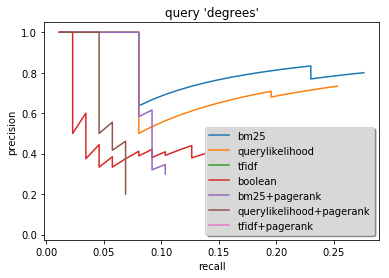
\includegraphics[width=\linewidth]{figure5}
        \caption{Precision/recall plot of query 'junwang'}
        \label{fig:junwang}
        \vskip -6pt
    \end{subfigure}%
    ~ 
    \begin{subfigure}{0.5\textwidth}
        \centering
        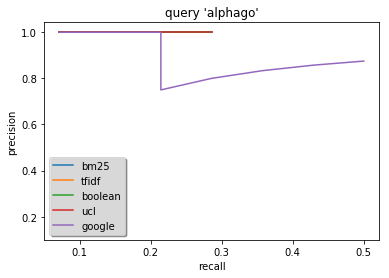
\includegraphics[width=\linewidth]{figure6}
        \caption{Precision/recall plot of query 'alphago'}
        \label{fig:alphago}
        \vskip -6pt
    \end{subfigure}
    \caption{Precision/recall curves for two example queries.}
\end{figure*}

Figure \ref{fig:junwang} and \ref{fig:alphago} show the precision and recall plots with the query 'AlphaGo' and 'junwang'. Due to there are too many models, we only plotted some of them with performances of google and ucl. It can be seen that every model could retrieve all documents relate to the query 'AlphaGo', while performance of each model varies significantly to the query 'junwang' although both queries are informational. The reason of this phenomenon is because the term 'AlphaGo' is still so new and unique that only a handful of pages that are actually using this term. Since the amount of documents in the collection that included the query 'AlphaGo' was only four documents, all of the models could easily retrieve them. In contrast, the term 'junwang' is much more general and popular, hence even non-relevant pages might include this term which would make it difficult for models to retrieve its relevant documents.

Table \ref{dcg} shows the DCG of performances of each of the algorithms with different types of queries. BM25 still has significantly better performance than the others, and we could easily interpret that BM25 is the best algorithm among those seven. Again, it can be seen that the DCG of the results from navigational queries is generally higher than informational queries, hence we could interpret this to that the metrics are also depending on the type of the query rather than only the specific ranking algorithm. Beside, BM25 does not perform well for every search term although it has a better overall performance than other models. For example, the term 'bioinformatics' was outperformed by the BMPG model.

\subsubsection{Ranking time}

Another aspect to take into consideration when evaluating performance of an algorithm is the time taken to rank the documents. Table \ref{time} shows the average time of 10 queries of different lengths, both with and without PageRank. These are delays observed by the end user, and could be shortened if running the search engine on the Amazon EC2 server, where it has faster access to the database.

Firstly, we can observe that BM25 spends considerably more time than the others. It is hard to explain the exact reason why it is spending almost double the time, but it might be caused by some implementation details where for example the database gets called more than usual. Query likelihood seems to perform better than TF-IDF overall as well. The Boolean ranking can be executed fastest of all. It can also be observed a small increase in the timing when applying PageRank to the queries. This can especially be seen for the query likelihood where the time was increased by 42\%.

% subsection analysis_of_results (end)

% section experiment (end)

\section{Discussion \& Limitations} % (fold)
\label{sec:discussion_&_limitations}

Different type of implementation of TF-IDF and BM25, but we have only chosen some. 
Our project has so far only considered a subset of existing algorithms. In order to get a wider picture of the different algorithms, it could be a good idea to include even more ranking algorithms. Also, some additional weighting algorithms could also be included in order to increase the accuracy of our results, such as HITS algorithm.

One of the major limitations in this project was circled around the crawler. The framework Scrapy was not written by us and we would not necessarily know that the crawler did exactly what we asked for. Scrapy retrieved lower amount of pages that expected and therefore made us question its quality. Since this was discovered relatively late, there were no time to try to get used to a new framework. Hence, when analysing the results it must be taken into consideration that the crawler might not have caught all the links in the CS domain. Also the problem with not crawling everything might have been because a max depth was set. Although the crawler indicated that it would take around 20 days without the depth, a further look into improving this should be made.

During the evaluation we had a limitation in our test set. The test set could be increased to compare even more queries, but because of time limitation we were not able to implement any more queries. This limits the credibility of our results, even though they are still sufficient to some extent.

Because of time restrictions, we also had to leave out a deep learning based ranking algorithm we were hoping to build. Although we do not have an implementation, we have a vision of how we wanted to design this ranker. It would be based on a deep neural network that would receive the scores of each of our 5 models, including PageRank, as input. To further increase the number of features, our second index with raw (unstemmed) document terms could be used, as well. The network would then weight the given scores appropriately such that its output rankings would match the labeled rankings of a training set as closely as possible. In this way, it would have been able to take advantage of the respective strengths of each of our algorithms while compensating for their individual weaknesses.

% section discussion_&_limitations (end)

\section{Conclusion} % (fold)
\label{sec:conclusion}

From our results, it can be concluded that our search engine behaves in a desirable way. It successfully retrieves relevant documents to our queries and BM25 managed to achieve precision results up to 70\%, as well as recall results up to 62\%. The goal of the project was to rank and compare different models, which has been achieved through both crawling, indexing and implementing five main algorithms. The four algorithms Boolean Retrieval, TF-IDF, BM25, Query Likelihood behaved in an expected manner according to previous work in the field. One surprising conclusion from the results was how PageRank didn't add any value to retrieving relevant documents, but instead decreased both precision and recall values for all the ranking algorithms. 

For future work we believe our deep learning assisted ranking could have been a novel contribution to the problem of IR, as no other model is likely to be built up of exactly our choice of features, and converge on the exact same weights in the training process, especially given our original test set. However, one limitation that would have made an application of deep learning difficult in our case was the manually defined set of test queries. When training a large neural network for the general task of ranking search results, a large amount of data is needed to achieve comparable performance on an unseen test set compared to the training set. A training set that is too small is highly likely to lead to over fitting instead. Furthermore, the requirement of an intimate connection to our evaluation metrics was another limiting factor in implementing the proposed method, as the evaluation is not fully packed in a standalone module and is largely based on independent notebook files.



% section conclusion (end)


